\documentclass[paper=letter, fontsize=11pt]{scrartcl} 
\usepackage{graphicx}
\usepackage{verbatim}
\usepackage{pictex}  
\usepackage{multimedia}
\usepackage{listings}
\usepackage{xcolor,colortbl}
\usepackage[utf8]{inputenc}		%para identificar acentos(encoding)
\usepackage{url}
\usepackage[spanish]{babel} % language/hyphenation
\usepackage{amsmath,amsfonts,amsthm} % Math packages
\usepackage{amsbsy}
\usepackage{amssymb}
\usepackage{fancyvrb}
\usepackage{sectsty} % Allows customizing section commands
\allsectionsfont{\centering \normalfont\scshape} % Make all sections centered, the default font and small caps
\usepackage{float}%para fijar las figuras y tablas
\usepackage{placeins}%fija espacios
\usepackage{fancyhdr} % Custom headers and footers
\pagestyle{fancyplain} % Makes all pages in the document conform to the custom headers and footers
\fancyhead{} % No page header - if you want one, create it in the same way as the footers below
\fancyfoot[L]{} % Empty left footer
\fancyfoot[C]{} % Empty center footer
\fancyfoot[R]{\thepage} % Page numbering for right footer
\renewcommand{\headrulewidth}{0pt} % Remove header underlines
\renewcommand{\footrulewidth}{0pt} % Remove footer underlines
\setlength{\headheight}{13.6pt} % Customize the height of the header

\numberwithin{equation}{section} % Number equations within sections (i.e. 1.1, 1.2, 2.1, 2.2 instead of 1, 2, 3, 4)
\numberwithin{figure}{section} % Number figures within sections (i.e. 1.1, 1.2, 2.1, 2.2 instead of 1, 2, 3, 4)
\numberwithin{table}{section} % Number tables within sections (i.e. 1.1, 1.2, 2.1, 2.2 instead of 1, 2, 3, 4)

\setlength\parindent{0pt} % Removes all indentation from paragraphs - comment this line for an assignment with lots of text

\newcommand{\horrule}[1]{\rule{\linewidth}{#1}} % Create horizontal rule command with 1 argument of height

\title{	
\normalfont \normalsize 
\textsc{Centro de Investigaci\'on en Matem\'aticas (CIMAT). Unidad Monterrey} 
\\ [25pt] 
\horrule{0.5pt} \\[0.4cm] % Thin top horizontal rule
\huge Tarea 1 \\ 
\horrule{2pt} \\[0.5cm] % Thick bottom horizontal rule
}

\author{José Antonio Garcia Ramirez} % Your name

\date{\normalsize\today} % Today's date or a custom date

\begin{document}
\lstdefinestyle{customc}{
  belowcaptionskip=1\baselineskip,
  basicstyle=\footnotesize, 
  frame=lrtb,
  breaklines=true,
  %frame=L,
  %xleftmargin=\parindent,
  language=C,
  showstringspaces=false,
  basicstyle=\footnotesize\ttfamily,
  keywordstyle=\bfseries\color{green!40!black},
  commentstyle=\itshape\color{red!40!black},
  identifierstyle=\color{blue},
  stringstyle=\color{purple},
}

\lstset{breakatwhitespace=true,
  basicstyle=\footnotesize, 
  commentstyle=\color{green},
  keywordstyle=\color{blue},
  stringstyle=\color{purple},
  language=C++,
  columns=fullflexible,
  keepspaces=true,
  breaklines=true,
  tabsize=3, 
  showstringspaces=false,
  extendedchars=true}

\lstset{ %
  language=R,    
  basicstyle=\footnotesize, 
  numbers=left,             
  numberstyle=\tiny\color{gray}, 
  stepnumber=1,              
  numbersep=5pt,             
  backgroundcolor=\color{white},
  showspaces=false,             
  showstringspaces=false,       
  showtabs=false,               
  frame=single,                 
  rulecolor=\color{black},      
  tabsize=2,                  
  captionpos=b,               
  breaklines=true,            
  breakatwhitespace=false,    
  title=\lstname,             
  keywordstyle=\color{blue},  
  commentstyle=\color{dkgreen},
  stringstyle=\color{mauve},   
  escapeinside={\%*}{*)},      
  morekeywords={*,...}         
} 


\maketitle % Print the title

\section{Ejericicio 1}
\textit{Considera los datos que se encuentran en el archivo} $wine\_quality.csv$, \textit{que contienen diferentes caractersticas sico-qumicas de las variantes tinto y blanco del} $Vinho$ \textit{Verde, un vino Portugues que cuenta con denominación de origen controlada. El archivo contiene 11 atributos (covariables) y una variable categorica (sensorial) que indica la calidad del vino en escala del 0 (muy malo) al 10 (excelente). Se agrego ademas una columna que identica el tipo de vino (tinto o blanco). Para mas detalles, consulta el archivo winequality.names.txt.}\\

\textit{Realiza un analisis exploratorio de los datos con las herramientas que consideres apropiadas. Comenta tus hallazgos. ¿Es posible distinguir el tipo de vino a partir de sus caractersticas físicoqumicas?}\\


El análisis exploratorio comenzó utilizando la herramienta ggobi para obtener una matriz de gráficos de dispersión con todas las variables (fisicoquímicas y la variable que indica el tipo de vino) a considerar seguido de un ‘Rotation’ (como lo denomina el software) ello dio pie a la idea de que distinguir el tipo de vino a partir de sus características fisicoquímicas o a una rotación de ellas es posible.
Posteriormente se aplicó la técnica de PCA sobre la matriz de correlación, de las variables mencionadas en el párrafo anterior, de donde la siguiente gráfica, donde se observa que las dos primeras componentes principales parecen resolver el problema de la separación.\\

\begin{figure}[htpb]
  \begin{center}
    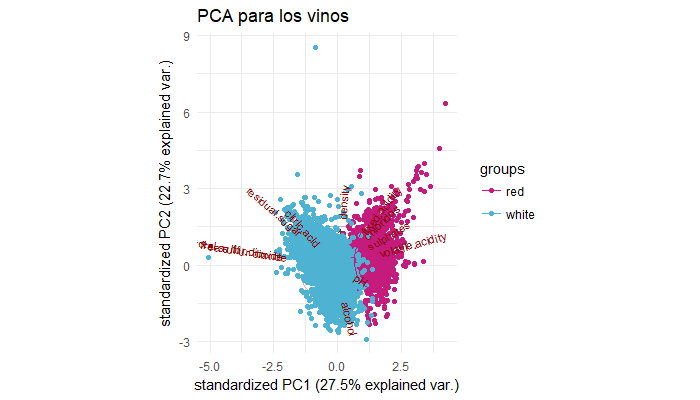
\includegraphics[scale=.6]{pca_vinos2.png}
    \caption{Biplot de la descomposición en componentes principales para los datos normalizados de los vinos}
    \label{fig:pca_vinos}
  \end{center}
\end{figure}
Es por ello por lo que considere un rankeo de las variables tomando el valor absoluto del loading que cada una de las 3 componentes le otorga y multiplicándolo por el porcentaje de varianza que explica la correspondiente componente principal. En donde las variables con mayor rankeo son 'total.sulfur.dioxide', 'residual.sugar' y 'fixed.acidity'. Después de graficar en 3d éstas variables normalizadas y no normalizadas se observa que la separación es más factible en la grafica que considera las variables originales.\\
\begin{figure}[htpb]
  \begin{center}
    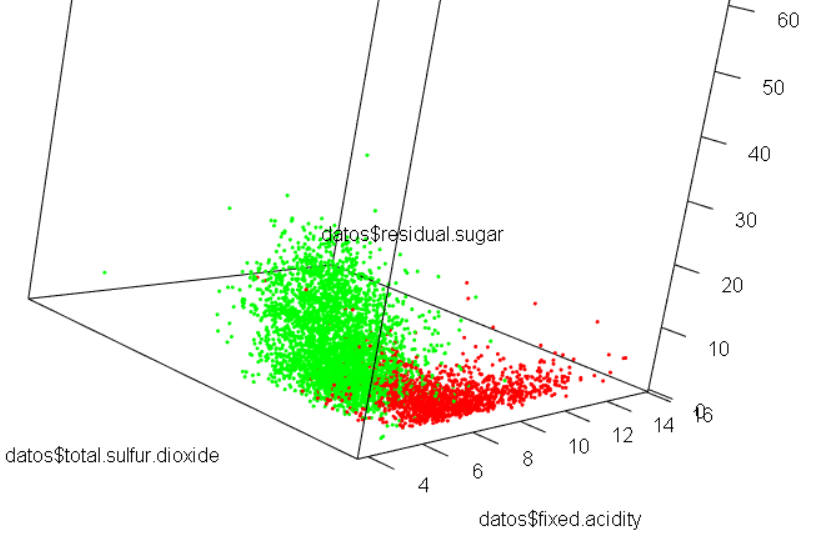
\includegraphics[scale=.35]{seleccion2.png}
    \caption{Visualización de las variables 'total.sulfur.dioxide', 'residual.sugar' y 'fixed.acidity' en su escala original. Los puntos rojos corresponden a vinos de tipo 'red' y los puntos verdes corresponden a vinos de tipo 'white'}
    \label{fig:selec_vinos}
  \end{center}
\end{figure}
\newpage
\textit{Un objetivo interesante es explorar la relacion entre las caractersticas medidas y la calidad del vino (tinto y blanco por separado). Verica si es posible encontrar visualmente tal relacion. Puedes simplicar o agrupar la escala de calidad en, por ejemplo, 3 categorias: malo, medio y excelente.}\\
Si bien con la ayuda del software ggbobi (y uso exhaustivo del mismo), existe una rotación de los datos que separa suficientemente bien para el caso del vino rojo, como se muestra en la siguiente gráfica, esto no implica que con las medidas realizadas sea posible sino con una rotación de éstas (en este caso no puedo recrear la rotación que realiza el software).
\begin{figure}[htpb]
  \begin{center}
    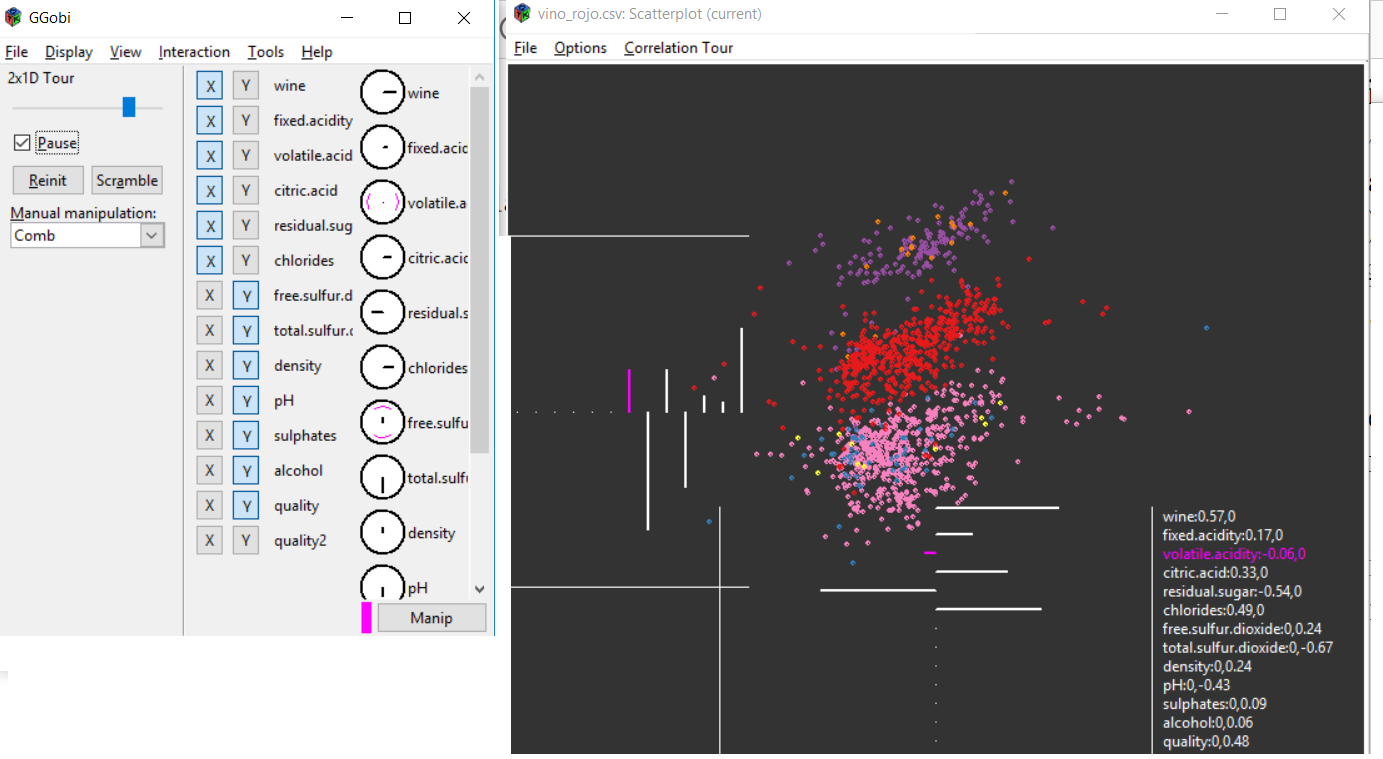
\includegraphics[scale=.35]{separacion_vino_rojo.png}
    \caption{Rotación efectuada por el software ggobi en donde es posible distinguir las 6 calificaciones de calidad (3,4,5,6,7 y 8).}
    \label{fig:separacion_vinos}
  \end{center}
\end{figure}

En vista de que no pude recrear la rotación de ggobi, utilice el mismo procedimiento que en el ejercicio anterior: rankeo las variables considerando el valor absoluto del loading que cada componente principal asigna (también considere los dos casos para cada tipo de vino PCA sobre la matriz de varianza-covarianza y sobre la matriz de correlación) y multiplicándolo por la varianza explicada por la misma componente (el parámetro del numero de componentes que usé fue de fuerza bruta es decir que hice el rankeo para todas las variables desde considerando solo la primer componente hasta la última componente principal), para al final retener y graficar las 3 variables con mejor rank.\\
Para los dos tipos de vino (rojo y blanco) agrupe la escala de calidad, para tener muestras balanceadas es decir con proporciones semejantes dentro del conjunto de datos; en el caso del vino rojo agrupe los valores 3,4 y 5 en 'malo', 6 para 'medio' y los restantes en 'excelente' (por el bajo numero de 7, 8, y 9 esta clase se mantuvo con 217 observaciones) mientras que para el vino blanco se agruparon los valores de la misma manera.\\
Para el vino rojo la mejor visualización la obtuve con las 3 primeras componentes principales empleando PCA sobre la matriz de varianza-covarianza y graficando las observaciones en su escala natural.\\

\begin{figure}[H]
  \begin{center}
    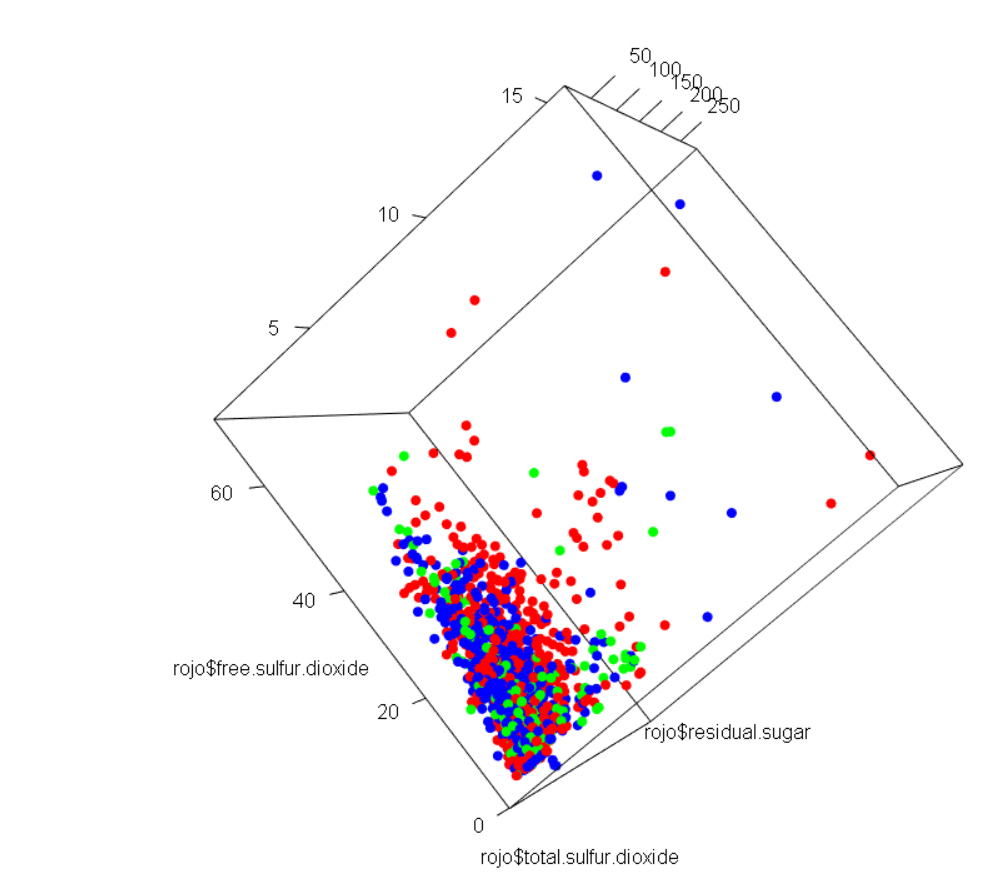
\includegraphics[scale=.3]{final_vino_rojo_sin_scalar.PNG}
    \caption{Las variables mejor rankeadas para el vino rojo fueron: $total.sulfur.dioxide$, $free.sulfur.dioxide$ y $residual.sugar$. El color rojo indica calidad 'malo', el azul calidad 'medio' y el verde calidad 'excelente'}
    \label{fig:separacion_vino_rojo}
  \end{center}
\end{figure}

Finalmente, para el vino blanco la mejor visualización la obtuve con las 3 primeras componentes principales empleando PCA sobre la matriz de correlación y graficando las observaciones escaladas.
\begin{figure}[H]
  \begin{center}
    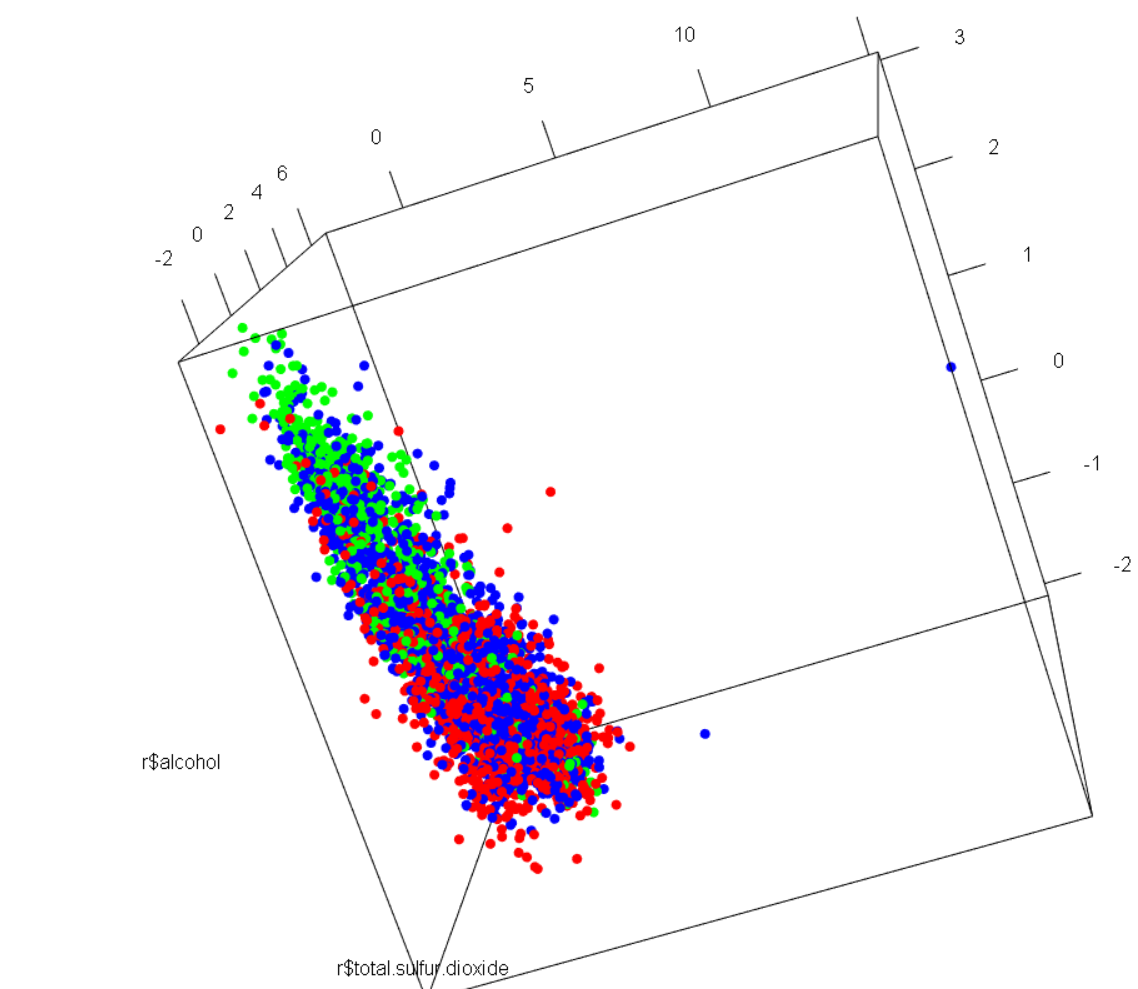
\includegraphics[scale=.20]{final_vino_blanco_checarcodigo.PNG}
    \caption{Las variables mejor rankeadas para l vino blanco fueron: $density$, $total.sulfur.dioxide$ y $alcohol$ (a diferencia de la gráfica anterior donde las variables selecionadas fueron otras). El color rojo indica calidad 'malo', el azul calidad 'medio' y el verde calidad 'excelente'}
    \label{fig:separacion_vino_blanco}
  \end{center}
\end{figure}

Por completes incluyo el código con el que trabaje:\\

\begin{lstlisting}[style=customc,basicstyle=\scriptsize]
datos <- read.csv('wine_quality.csv')
datos$quality <- factor(datos$quality)
data <- datos[ ,2:12]#no considero la variable 'quality'
a <- scale(data)
a <- as.data.frame(a)
pca <- princomp(a)
a$wine <- datos$wine
a$color <- 'red'
index <- which(as.character(a$wine) != 'red') 
a$color[index] <- 'green'
a$wine <- datos$wine
round(cumsum(pca$sdev**2/sum(pca$sdev**2)),2)
componentes <- pca$loadings
rankeo <- abs(componentes[,1:3])%%#esta es multiplicacion de matrices pero el tex no lo reconoce
matrix(pca$sdev**2/sum(pca$sdev**2))[1:3]**2, nrow = 3)
rankeo <- as.data.frame(rankeo)
rankeo$variable <- row.names(rankeo)
rankeo <- rankeo[order(rankeo$V1, decreasing = TRUE),]
head(rankeo,3) #las tres variables con las que se decidio ilustrar 
data.rotada <- pca$scores
data.rotada <- as.data.frame(data.rotada)
data.rotada$wine <- datos$wine
library(ggbiplot)
pca.vinos <- ggbiplot(pca, groups = datos$wine,ellipse = TRUE, circle = TRUE)+
  scale_color_manual(values=c('#C51B7D','#4EB3D3'))+
  theme_minimal( ) + ggtitle("PCA para los vinos")
library(rgl)
datos$color <- a$color
plot3d(a$residual.sugar, a$fixed.acidity, a$total.sulfur.dioxide, col = a$color)
plot3d(datos$residual.sugar, datos$fixed.acidity, datos$total.sulfur.dioxide, col = datos$color)
################## sub problemas 
rojo <- subset(datos, wine=='red')
rojo$quality2 <- as.character(rojo$quality)
sum(table(rojo$quality))/3
levels(rojo$quality) <- c('malo', 'malo', 'malo', 'medio', 'excelente', 'excelente', 'excelente')
table(rojo$quality)
r <- scale(rojo[, 2:12])
r <- as.data.frame(r)
r$quality <- rojo$quality
r$quality2 <- as.character(rojo$quality2)
blanco <- subset(datos, wine=='white')
blanco$quality2 <- blanco$quality
sum(table(blanco$quality))/3
levels(blanco$quality) <- c('malo', 'malo', 'malo', 'medio', 'excelente', 'excelente', 'excelente')
table(blanco$quality)
pca.rojo <- princomp((rojo[, 2:12]))
pca.rojo
plot(pca.rojo)
cumsum(pca.rojo$sdev**2/sum(pca.rojo$sdev**2))
rankeo.rojo <- abs(pca.rojo$loadings[,1:3])* #esta es multiplicacion de matrices pero el tex no lo reconoce matrix((pca.rojo$sdev**2/sum(pca.rojo$sdev**2))[1:3]**2, nrow = 3)
rankeo.rojo <- as.data.frame(rankeo.rojo)
rankeo.rojo$variable <- row.names(rankeo.rojo)
rankeo.rojo <- rankeo.rojo[order(rankeo.rojo$V1, decreasing = TRUE),]
head(rankeo.rojo,3) #las tres variables con las que se decidio ilustrar
colors <- list(malo='red', medio='blue', excelente='green')
plot3d(  rojo$total.sulfur.dioxide, rojo$free.sulfur.dioxide, rojo$residual.sugar, col = unlist(colors[rojo$quality]), size = 8)
##########
pca.blanco <- princomp(scale(blanco[, 2:12]))
plot(pca.blanco)
cumsum(pca.blanco$sdev**2/sum(pca.blanco$sdev**2))
rankeo.blanco <- abs(pca.blanco$loadings[,1:3])*#esta es multiplicacion de matrices pero el tex no lo reconoce matrix((pca.blanco$sdev**2/sum(pca.blanco$sdev**2))[1:3]**2, nrow = 3)
rankeo.blanco <- as.data.frame(rankeo.blanco)
rankeo.blanco$variable <- row.names(rankeo.blanco)
rankeo.blanco <- rankeo.blanco[order(rankeo.blanco$V1, decreasing = TRUE),]
head(rankeo.blanco,3) #las tres variables con las que se decidio ilustrar 
#plot3d( blanco$density, blanco$total.sulfur.dioxide, blanco$alcohol, col = unlist(colors[blanco$quality]), size = 8)
r <- scale(blanco[, 2:12])
r <- as.data.frame(r)
plot3d( r$density, r$total.sulfur.dioxide, r$alcohol, col = unlist(colors[blanco$quality]), size = 8)
\end{lstlisting} 

\section{Ejercicio 2}
\begin{enumerate}
\item Realiza PCA a la matriz\\
\[
\Sigma = \begin{pmatrix}
			1 & \rho \\
            \rho & 1 \end{pmatrix}
\]
Donde $\rho > 0$.\\
Primero calculamos los valores propios con el polinomio característico de $\Sigma$\\
\[
p_{\Sigma}(\lambda) = det(\Sigma - \lambda 1) = \begin{vmatrix}
			1 - \lambda & \rho \\
            \rho & 1 -\lambda \end{vmatrix} =\lambda^2 -2\lambda+(1-\rho^2)
\]
Cuyas soluciones están dadas por:

\[
\lambda= \frac{2\pm \sqrt{4-4(1-\rho^2}}{2} = 1 \pm \sqrt{p^{2}} = 1 \pm \rho 
\]
Como $\rho>0$ el valor propio $1+\rho$ es el que corresponde al primer componente principal, calculemos el vector propio asociado a este valor propio.
\[
\Sigma - (1+\rho)1 = \begin{pmatrix}
					1- (1+\rho) & \rho \\
                    \rho & 1- (1+\rho)
                    \end{pmatrix}
                    = \begin{pmatrix}
					-\rho & \rho \\
                    \rho & -\rho
                    \end{pmatrix} \sim 
                    \begin{pmatrix}
					0 & 0 \\
                    \rho & -\rho
                    \end{pmatrix}
\]
De donde el vector $(1,1)^t$ es el vector propio asociado a $(1+\rho)$, si lo normalizamos tenemos que la primer componente principal está dada por $(1/ \sqrt{2}, 1/ \sqrt{2})$.
De manera análoga para el valor propio $(1-\rho)$ tenemos:\\
\[
\Sigma - (1-\rho)1 = \begin{pmatrix}
					1- (1-\rho) & \rho \\
                    \rho & 1- (1-\rho)
                    \end{pmatrix}
                    = \begin{pmatrix}
					\rho & \rho \\
                    \rho & \rho
                    \end{pmatrix} \sim 
                    \begin{pmatrix}
					0 & 0 \\
                    \rho & \rho
                    \end{pmatrix}
\]
Entonces el vector $(1,-1)^t$ es el vector propio asociado a $(1+\rho)$, si lo normalizamos tenemos que la segunda componente principal esta dada por $(1/ \sqrt{2}, -1/ \sqrt{2})^t$.\\\\

\textit{Ahora, cambia la escala de $X_1$, es decir, considera la covarianza de} $cX_1$ y $X_2$. \textit{¿Cómo cambian los componentes principales al realizar este escalamiento?}\\\\
En principio si $\Sigma $ denota una matriz de correlaciones es inmediato ver que el escalamiento no afecta a las componentes pues 
\[corr(cx_1,x_2) = \frac{cov(cx_1,x_2)}{\sigma_{cx_1}\sigma_{x_2}}= \frac{c*cov(x_1,x_2)}{\sigma_{cx_1}\sigma_{x_2}}\]
y como $\sigma_{cx_1}= \sqrt{var(cx_1)}=\sqrt{c^2var(x_1)}= c \sigma_{x_1}$
entonces $corr(cx_1,x_2)= \frac{c*cov(x_1,x_2)}{\sigma_{cx_1}\sigma_{x_2}} = \frac{c*cov(x_1,x_2)}{c\sigma_{x_1}\sigma_{x_2}}=corr(x_1,x_2)=\rho$\\

En el caso en que $\Sigma$ sea una matriz de varianza-covarianza sí cambia este escalamiento como lo muestran los siguientes cálculos, sabemos que si $\rho=cov(x_1,x_2)$ entonces $cov(cx_1,x_2)=c*cov(x_1, x_2)=c\rho$ por lo que $\Sigma$ cambia a la forma 

\[
\Sigma  = \begin{pmatrix}
					c^2  & c\rho \\
                    c\rho & 1
                    \end{pmatrix}
\]
Cuyo polinomio característico esta dado por $p_{\Sigma}(\lambda)=\lambda^2-\lambda(c^2+1) +c^2 -c^2\rho^2$ \\
Cuyas raíces son de la forma:
\[
 \lambda = \frac{(c^2+1) \pm \sqrt{ (c^2 +1)^2+4c^2(\rho^2 -1)) } }{2} 
\]

Que siempre existen porque el discriminante siempre es positivo aun cuando la correlación sea negativa y aun cuando $c<0$, además como estos son valores propios de una matriz simétrica es un resultado que siempre son reales.\\

Para obtener los vectores propios consideremos la matriz $\Sigma -\alpha1$, donde $\alpha$ es el valor propio correspondiente al primer componente principal 
\[
 \alpha = \frac{(c^2+1) + \sqrt{ (c^2 +1)^2+4c^2(\rho^2 -1)) } }{2} 
\]
Entonces 
\[
\Sigma -\alpha1 =\begin{pmatrix}
					c^2 -\alpha & c\rho \\
                    c\rho & 1-\alpha
                    \end{pmatrix}
\]
Como $\alpha$ es un valor propio sabemos que la matriz anterior induce el sistema de ecuaciones 
\begin{equation}
(c^2 -\alpha )x_1 + c\rho x_2 = 0
\end{equation}
\begin{equation}
c\rho x_1 + (1-\alpha)x_2 = 0
\end{equation}
Multiplicando por $-1$ las dos ecuaciones anteriores e igualándolas tenemos 
\begin{equation*}
(\alpha - c^2) x_1 -c\rho x_2 = -c\rho x_1+(\alpha-1)x_2
\end{equation*}
De donde podemos obtener la dirección de la componente principal al notar que 
\[
\frac{\alpha-c^2+c\rho}{\alpha-1+c\rho}x_1 = x_2
\]
Es decir que la primer componente principal es el vector :\\
\[ 
P_1 = 
\left(\sqrt{ 1 + \left(\frac{\alpha-c^2+c\rho}{\alpha-1+c\rho}\right)^2 }\right)^{-1} 
\begin{pmatrix}
1 \\
\frac{\alpha-c^2+c\rho}{\alpha-1+c\rho}
 \end{pmatrix}
\]

Donde la segunda componente (del vector) está bien definida porque $\alpha-1+c\rho$ nunca se hace cero como lo podemos comprobar con los casos extremos en que $c\rho<0$ se tendría 

\[
\begin{split}
\alpha -1 -c \rho & =\frac{(c^2+1) + \sqrt{ (c^2 +1)^2 + 4c^2(\rho^2 -1) }}{2}-1-c\rho \\
&= c^2 /2 -c \rho +  \sqrt{ (c^2 +1)^2 + 4c^2(\rho^2 -1) }/2 -1/2
\end{split}
\]
Y como $c^2/2>cp$ y $\sqrt{ (c^2 +1)^2 + 4c^2(\rho^2 -1) }/2 >1/2$, entonces la primer componente esta bien definida.\\
Aprovechando el hecho de que los vectores propios son perpendiculares entonces 
La segunda componente principal es:
\[ 
P_2 = 
\left(\sqrt{ 1 + \left(\frac{\alpha-c^2+c\rho}{\alpha-1+c\rho}\right)^2 }\right)^{-1} 
\begin{pmatrix}
-\frac{\alpha-c^2+c\rho}{\alpha-1+c\rho}\\
1
 \end{pmatrix}
\]
Como podemos ver de las formas explicitas de las componentes principales, el escalamiento sí afecta la dirección de las componentes así como sus respectivos $loadings$ o pesos que asignan a cada variable.\\
Notemos además que éste caso es una generalización del anterior pues cuando $c = \rho = 1$ se obtiene que la primer componente principal es de la forma 
\[P_1 = \left(\sqrt{ 1 + \left(\frac{\alpha-c^2+c\rho}{\alpha-1+c\rho}\right)^2 }\right)^{-1} 
\begin{pmatrix}
1 \\
\frac{\alpha-c^2+c\rho}{\alpha-1+c\rho}
 \end{pmatrix}
 = \frac{1}{\sqrt{2}} \begin{pmatrix}
1\\ 1  \end{pmatrix}\] Y la segunda componente principal queda de la forma \[ 
P_2 = 
\left(\sqrt{ 1 + \left(\frac{\alpha-c^2+c\rho}{\alpha-1+c\rho}\right)^2 }\right)^{-1} 
\begin{pmatrix}
-\frac{\alpha-c^2+c\rho}{\alpha-1+c\rho}\\
1
 \end{pmatrix} = \frac{1}{\sqrt{2}} \begin{pmatrix}
-1\\
1
\end{pmatrix}
\]
Como en el caso anterior.
\item
\textit{Considera los datos del archivo \textbf{ushealth.csv}, que contiene el número reportado de muertes en los 50 estados de los Estados Unidos, clasicado de acuerdo a 7 categorias: accidentes \textbf{acc}, cardiovascular \textbf{card}, cáncer \textbf{canc}, pulmonar \textbf{pul},
neumonia \textbf{pneu}, diabetes \textbf{diab} y enfermedades del hígado \textbf{liv}.}\\
\textit{Realiza PCA, con y sin normalización e interpreta los resultados. ¿Qué puedes decir sobre la relación entre las causas y el número de muertes? Usa el resultado del inciso anterior para explicar el efecto de usar PCA normalizado y sin normalizar. ¿Cuál prefieres usar en este caso y porque? ¿Qué recomendación darías al respecto al usar PCA en general? }\\
Al realizar PCA sobre los datos sin escalar, se obtiene que la primer componente principal explica aproximadamente el\textbf{ 96\% de la variación total}, \textbf{lo cual es extrañamente sospechoso} puesto que reducir dimensión es el objetivo de este método la reducción debe mantenerse informativa. \\

Al observar los pesos o loadings de la primer componente obtenida sin normalizar los datos vemos que esta componente da un gran peso (negativo) a las variables 'card' y 'canc' y un peso pequeño (en comparación de las dos anteriores) a todas las demás. En particular esta componente solo otorga un peso positivo a la variable 'acc' lo cual es natural puesto que desde la matriz de varianzas y covarianzas esta variable se correlaciona negativamente con todas las demás.\\
En el siguiente biplot que mostramos es difícil apreciar las direcciones de las variables que no sean 'card' y 'canc' respaldando lo dicho en el párrafo anterior.
\begin{figure}[H]
  \begin{center}
    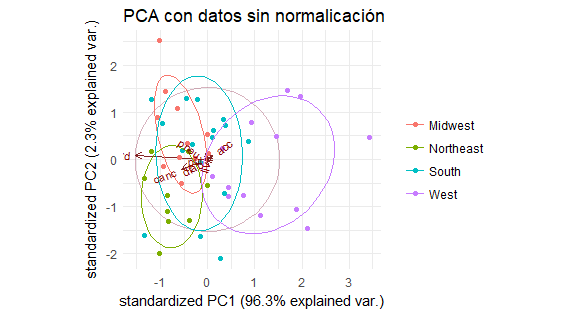
\includegraphics[scale=.95]{pca_sin_normalizar.png}
    \caption{Biplot de la descomposición en componentes principales para los datos sin normalizar, los colores indican la región en donde se ubica el estado   }
    \label{fig:pca_sin}
  \end{center}
\end{figure}
Al normalizar los datos, restar media y dividir entre la desviación estándar de cada variable, se obtuvó que en contraste al ejercicio anterior la primer componente solo explica el 48\% de la variación total en el conjunto de datos, de hecho para cubrir 90\% de la variación total se requiere de las cuatro primeras componentes.\\

Al igual que en el ejercicio anterior la primer componente asigna un peso positivo a la variable 'acc' (hecho que se ve debe a que la correlación de esta variable con todas las demás es negativa)  y negativo a todas las demás (análogamente las variables 'card' y 'canc' son las que mantienen los loadings más grandes en magnitud pero en contraste al ejercicio anterior las demás variables 'pul', 'pneu', 'diab' y 'liv' tienen cargas de magnitud considerable pues ninguna de ellas es tres veces menor a la carga mayor otorgada a la variable 'card'.\\
En el siguiente biplot que mostramos es fácil apreciar las direcciones de las variables las demás variables puesto que sus pesos en las dos primeras componentes son significativos.
\FloatBarrier
\begin{figure}[H]
  \begin{center}
    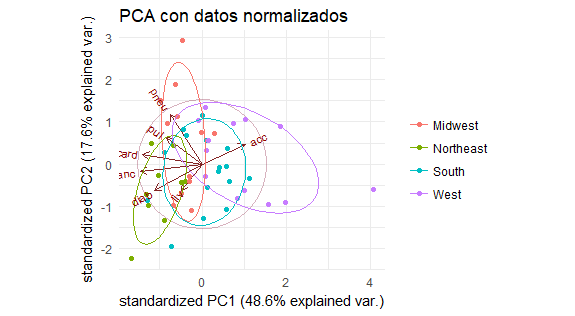
\includegraphics[scale=.95]{pca_con_normalizacion.png}
    \caption{Biplot de la descomposición en componentes principales para los datos normalizados, los colores indican la región en donde se ubica el estado   }
    \label{fig:pca_sin}
  \end{center}
\end{figure}

En conclusión, las causas y el número de muertes se correlacionan positivamente a excepción de las muertes por accidente las cuales se correlacionan en sentido contrario a las demás, esto lo notamos tanto en la matriz de varianza-covarianza, en la matriz de correlación es más notorio este hecho y esta información se ve reflejada en la primer componente principal de los datos (con y sin escalamiento).\\
Para este caso (y en general) prefiero usar PCA sobre la matriz de correlaciones (i.e. con los datos escalados) puesto que, aunque no reduce dimensión tanto (como en el caso en que los datos no se escalaron y una única componente explica más del 96\% de la variación) lo hace y mantiene coherencia y utilidad si usamos las primeras cuatro componentes.\\
Para concluir este ejercicio yo recomiendo realizar PCA sobre la matriz de correlaciones pues entre las variables pueden existir escalas y unidades diferentes y ello puede que altere el análisis.\\
Incluyo el código que utilicé solo por completes.
\begin{lstlisting}[style=customc,basicstyle=\scriptsize]
datos <- read.csv('ushealth.csv')
muertes <- datos[, 4:10 ]
pca.sin.normalizar <- princomp(x=muertes)
plot(cumsum(pca.sin.normalizar$sdev**2/sum(pca.sin.normalizar$sdev**2)), type='b')
abline(h = .98, col ='red')
pca.sin.normalizar$sdev**2/sum(pca.sin.normalizar$sdev**2)
round(pca.sin.normalizar$loadings[,"Comp.1"],4)
library(ggbiplot)
p1 <- ggbiplot(pca.sin.normalizar, groups = datos$reg,ellipse = TRUE, circle = TRUE)+
         scale_color_discrete(name = '') +
           theme_minimal( ) + ggtitle("PCA con datos sin normalicacion")
##############
cor(muertes)
muertes.scaladas <- scale(muertes)
pca.con.normalizacion <- princomp(muertes.scaladas)
plot(pca.con.normalizacion, type='l')
plot(cumsum(pca.con.normalizacion$sdev**2/sum(pca.con.normalizacion$sdev**2)), type='b')
abline(h = .8, col='red')
cumsum(pca.con.normalizacion$sdev**2/sum(pca.con.normalizacion$sdev**2))
round(pca.con.normalizacion$loadings[,"Comp.1"],4)
round(pca.con.normalizacion$loadings[,"Comp.2"],4)
p2 <- ggbiplot(pca.con.normalizacion, groups = datos$reg,ellipse = TRUE, circle = TRUE)+
  scale_color_discrete(name = '') +
  theme_minimal( ) + ggtitle("PCA con datos normalizados")
\end{lstlisting} 



\end{enumerate}

\section{Ejercicio 3}
\textit{Supón que un miembro del gabinete del gobierno de Nuevo León quiere plantear una estrategia de desarrollo social en el estado. Para esto, ha visto los últimos índices de marginación de Nuevo Leon y ha subrayado dos cosas: 1) no entiende como los calcularon y 2) le gustaría explorar otra forma de hacerlo. Para esto, esta buscado
personas que puedan ayudarlo a analizar la informacion (!seguro que pagan muy bien!). }\\
\begin{enumerate}
\item Trata de reproducir los resultados del índice de marginación a nivel localidad para el estado de NL. Para esto, utiliza los datos del Censo de Población y Vivienda 2010 reportados en el INEGI, los cuales, para facilitarte la tarea, he concentrado y adecuado en el archivo $censo\_nl.csv$. El diccionario de las variables del
censo puedes verlos en $diccionariodatosscince.pdf$. Los resultados reportados por la CONAPO se encuentran en el archivo $conapo\_marginacion\_nl.xls$. Realiza un reporte ejecutivo (facíl de entender), explicando
los resultados y la metodología usada. Agrega apéndices tecnicos a tu reporte si lo consideras necesario 2.\\
\subsection{Un conciso resumen sobre la construcción índice de marginación a nivel localidad para el estado de Nuevo León}

A nivel nacional el índice de marginación\footnote{La marginación se concibe como un problema estructural de la sociedad, en donde
no están presentes ciertas oportunidades para el desarrollo, ni las capacidades para
adquirirlas, ello pone en riesgo a la población con vulnerabilidades que les impiden alcanzar determinadas condiciones de vida.} a nivel localidad \footnote{El término localidad suele emplearse de manera indistinta para hacer mención a un municipio o a una zona urbana dentro de una ciudad} que calcula la CONAPO (desde 1990) es una forma de medir las carencias que padece la población como resultado de la falta de acceso a la educación, la residencia en viviendas inadecuadas y la carencia de bienes.% Su objetivo es por un lado contribuir a mostrar las disparidades territoriales que existen entre las localidades del país (estamos particularmente interesados en el estado de Nuevo León) y mostrar las relaciones existentes en el rubro de marginación entre entidades federativas y municipios, para ser utilizado en las reglas de operación de diversos programas de atención social.\\
Busca establecer un parámetro analítico que permita entender cuándo un sector de la sociedad se encuentra en una situación donde no están presentes las oportunidades para el desarrollo. Con el fin de detonar una discriminación positiva: los sectores beneficiarios logran, por medio de políticas públicas una forma de atraer y optimizar los recursos del estado para beneficio de la población. Por las variables del censo que utiliza para construirse este índice dice cuales \textbf{ubicaciones geográficas (localidades) están marginadas (y a qué nivel)}.
 \subsubsection{Construcción del índice de marginación por localidad.}
 \textbf{El índice de marginación por localidad es sencillamente una suma ponderada de ocho variables} que se construyen con datos que se extraen del censo del INEGI (en este caso reproducimos la estimación del índice para el estado de Nuevo León \footnote{Véase el anexo A para ver como se obtuvieron los datos.}. \\
Los números que funcionan como ponderadores (o factores de peso en términos de interpretabilidad) están dados por la metodología estadística concerniente a componentes principales (PCA por sus siglas en inglés)\footnote{Véase anexo B para seguir la reconstrucción del índice.}.\\
Primero las variables con las que se construye el índice cubren tres dimensiones (Educación, Vivienda y Disponibilidad de bienes). En cada dimensión se utilizan diversos 
indicadores socioeconómicos empleados para su medición, los cuales se miden en sentido privativo, es decir, como déficits y a su vez estos indicadores se (que son las variables que se ponderan) se construyen con datos del censo del INEGI.\\
A continuación, se enlistan las dimensiones mencionadas y sus indicadores respectivos:
\begin{enumerate}
\item Educación \\ 
Esta dimensión se integra por dos indicadores. El primero se relaciona con la capacidad
de las personas de leer y escribir un recado y prácticamente trunca toda posibilidad de adquirir conocimientos tanto en el sistema educativo ortodoxo, como de manera autodidacta. El segundo indicador se refiere al cúmulo mínimo de conocimientos específicamente a la compleción de la primaria. 
\begin{itemize}
\item Porcentaje de población de 15 años o más analfabeta. La abreviamos como $P_1$.
\item Porcentaje de población de 15 años o más sin primaria completa. La abreviamos como $P_2$.
\end{itemize}

\item Vivienda\\
La vivienda es el único espacio físico constante durante las etapas de la vida de los individuos,
desde la infancia hasta la edad adulta en plenitud, por lo que es determinante
para el desarrollo de capacidades, habilidades, madurez emocional y conocimientos
de toda persona. Explorar las condiciones de las viviendas resulta
esencial al tratar la marginación. Los cinco indicadores socioeconómicos considerados
en la dimensión vivienda son:
\begin{itemize}
\item Porcentaje de viviendas particulares habitadas sin excusado. La abreviamos como $P_3$.
\item Porcentaje de viviendas particulares habitadas sin energía eléctrica. La abreviamos como $P_4$.
\item Porcentaje de viviendas particulares habitadas sin agua entubada. La abreviamos como $P_5$.
\item Promedio de ocupantes por cuarto en viviendas particulares habitadas. La abreviamos como $P_6$.
\item Porcentaje de viviendas particulares habitadas con piso de tierra. La abreviamos como $P_7$.
\end{itemize}

\item Disponibilidad de bienes\\
Para considerar un indicador relativo a los ingresos por trabajo se decidió incluir la disponibilidad de refrigerador en las viviendas. La disponibilidad de refrigerador se encuentra condicionada por el ingreso
del que se dispone en las viviendas además el no tener refrigerador limita las posibilidades de contar con alimentos perecederos frescos e incrementa los riesgos de salud asociados con la
ingesta de alimentos con algún grado de descomposición y con una dieta deficiente.
En virtud de lo anterior, se considera el siguiente indicador socioeconómico:

\begin{itemize}
\item Porcentaje de viviendas particulares habitadas que no disponen de refrigerador.La abreviamos como $P_8$.
\end{itemize}
Entonces el índice de marginación por localidad es una suma ponderada de la forma:    
\[\begin{split} 
indice\_de\_marginacion\_por\_localidad& =0.379*P_1 + 0.370*P_2+0.323*P_3 + \\
& 0.366*P_4+ 0.266*P_5 + 0.327*P_6+\\
&0.366*P_7+ 0.413*P_8 \\
\end{split}
\]
Donde los valores que multiplican a los indicadores $P_i$ se obtienen al emplear el método estadístico de PCA sobre los datos de la encuesta del INEGI (2010). Véase el apéndice B para ver la reconstrucción del método empleado.\\
%%%%%%%%%%%%%%%%%
De donde podemos concluir que las variables $P_8,P_1 $ y $  P_2$ que corresponden a los índices ‘Porcentaje de viviendas habitadas que no disponen de refrigerador’, ‘Porcentaje de población de 15 años o más analfabeta’ y ‘Porcentaje de población de 15 años o más sin primaria completa’ respectivamente son en orden de importancia las más relevantes.

\subsubsection{Anexo A: Obtención de los datos del censo efectuado por el INEGI para 2010, para el estado de Nuevo León.}
Previamente se disponía de un subconjunto de datos del Censo de Población y Vivienda 2010 reportados en el INEGI, exclusivos del estado de Nuevo León (véase archivo $censo\_nl.csv$ el cual consultarse en la dirección \url{ https://github.com/fou-foo/MCE/blob/master/Second/CienciaDeDatos/tarea1/censo_nl.csv})  , que contiene la mayoría de las variables para construir los indicadores mientras que para complementar los datos necesarios se requirió de  realizar una búsqueda en el sitio del INEGI (\url{http://www3.inegi.org.mx/sistemas/iter/default.aspx}) y después de seleccionar las variables: 
\begin{itemize}
\item P15mas.sin.escolaridad
\item 15mas.con.primaria.incompleta 
\item P15mas.con.primaria.completa 
\item P15mas.con.secundaria.incompleta
\item P15mas.con.secundaria.completa 
\item P18mas.con.post
\item $VIV5\_R$ 
\item VIV6.complemento 
\item $VIV6$
\end{itemize}
Con lo que se construyo el archivo $VIV5\_R.csv$\footnote{Véase el anexo D para el diccionario de datos que se terminó usando para la reproducción de los resultados del índice de marginación a nivel localidad para el estado de Nuevo León y la respectiva comprobación con lo reportado por la CONAPO en su sitio web.} disponible en la dirección \url{https://github.com/fou-foo/MCE/blob/master/Second/CienciaDeDatos/tarea1/VIV5_R.csv}. El cruce entre los archivos se realiza con la columna $CVEGEO$\footnote{La variable se construyó concadenando la clave del estado, la clave del municipio a 3 cifras y la clave de la localidad a cuatro cifras.}.
\subsubsection{Anexo B: Reproducción de los resultados del índice de marginación a nivel localidad para el estado de Nuevo León}
A continuación recreamos la estimación efectuada por la CONAPO para el cálculo del índice de marginación por localidad, siguiendo el anexo C del documento principal disponible en \url{ http://www.conapo.gob.mx/en/CONAPO/Indice_de_Marginacion_por_Localidad_2010}.\\ 
Es importante notar que en la recreación realizada en ésta estimación \textbf{se trabaja con una muestra de menor tamaño} que la de la CONAPO, pues ellos en su momento calcularon el índice a nivel nacional y nuestra recreación es solo con las localidades del estado de Nuevo León y con datos provenientes del INEGI,\textbf{ por lo que se observarán variaciones}, sin embargo la misma CONAPO reporta los índices que construye, en su sitio web mencionado anteriormente, aprovechando esta otra fuente de datos en el anexo C se validan los coeficientes de la primer componente principal así como otros estadísticos a nivel nacional.\\
Una vez que se dispone de los datos que recabamos según el anexo A (archivos $censo\_nl.csv$ y $VIV5\_R.csv$) y  la información contenida en el anexo C del sitio de la CONAPO anteriormente referenciado comenzamos a construir los indicadores mencionados en el apartado 3.1.1\footnote{El diccionario de datos empleado en esta recreación se encuentra en el anexo D.}\\
Después de efectuar el join (o cruce de tablas) entre la información contenida en nuestros dos archivos que contienen la información del censo del INEGI 2010\footnote{Utilizando como llave el campo $CVEGEO$ resultan las 2037 observaciones reportadas en el 'Cuadro C.2. Localidades y población total por entidad federativa, 2010' del anexo C del documento principal en el sitio referenciado previamente de la CONAPO} podemos construir los indicadores para el estado de Nuevo León de acuerdo al anexo C del documento principal referenciado en el sitio web de la CONAPO, previo a lo anterior se efectuó una imputación de datos sencilla, reemplazando en todas las variables los datos menores a cero por cero excepto en los casos de las varables$POB20, VIV16,VIV14$ y $VIV24$ donde los valores negativos se cambiaron por la unidad (considerando que son poblaciones en localidades están deben de ser cuando menos mayor o igual a cero, sin embargo para fines prácticos este conjunto de variables definen cocientes por lo cual conviene igualarlos por 1 que es la menor cantidad positiva mayor a cero en nuestras unidades observables, es decir personas).\begin{itemize}
\item Para el porcentaje de población de 15 años o más analfabeta el cálculo de este indicador se realizó mediante la división de la población de 15 años o más analfabeta entre el total de la población de 15 años o más es decir \\
\[P_1 = 100*\frac{EDU28}{POB20}
\].
\item Porcentaje de población de 15 años o más sin primaria completa. 
\[ 
P_2 = \text{\tiny{\( 100*\frac{P15.sesc + P15cpri.inc}{
            P15.sesc + P15cpri.inc + 
               P15cpri.com	+ P15csec.inc +
               P15csec.com + P18.c.post} \)} } \]    

\item Porcentaje de viviendas particulares habitadas sin excusado. 
\[
P_3 = 100\frac{VIV2-VIV19}{VIV2}
\]
\item Porcentaje de viviendas particulares habitadas sin energía eléctrica. 
\[
P_4 = 100\frac{VIV15}{VIV14+VIV15}
\]
\item Porcentaje de viviendas particulares habitadas sin agua entubada. 
\[
P_5 = 100\frac{VIV17}{VIV16+VIV17}
\]
\item Promedio de ocupantes por cuarto en viviendas particulares habitadas.
\[
P_6 = log(VIV5_R)
\]
\item Porcentaje de viviendas particulares habitadas con piso de tierra. 
\[
P_7 = 100\frac{VIV6}{VIV6 + VIV6.complemento}
\]
\item Porcentaje de viviendas particulares habitadas que no disponen de refrigerador.
\[
P_8 = 100\frac{VIV2-VIV26}{VIV2}
\]
\end{itemize}
Los estadísticos descriptivos calculados con los datos del censo del INEGI 2010 contra los que reporta la CONAPO se resumen en la siguiente tabla:
\begin{table}[ht]
\centering
\begin{tabular}{rrrrrrrrrrrl}
  \hline
 & Rango & RanCona & Mín & MínCona & Máx & MáxCona & Media & MedCona & Sd & SdCona  \\ 
  \hline
P1 & 77.78 & 77.78 & 0.00 & 0.00 & 77.78 & 77.78 & 6.11 & 9.01 & 9.68 & 9.72  \\ 
  P2 & 100.00 & 100.00 & 0.00 & 0.00 & 100.00 & 100.00 & 39.32 & 39.32 & 19.25 & 19.25 \\ 
  P3 & 100.00 & 100.00 & 0.00 & 0.00 & 100.00 & 100.00 & 14.79 & 10.39 & 28.05 & 17.90 \\ 
  P4 & 96.97 & 100.00 & 0.00 & 0.00 & 96.97 & 100.00 & 5.20 & 9.10 & 18.52 & 22.76  \\ 
  P5 & 99.73 & 100.00 & 0.00 & 0.00 & 99.73 & 100.00 & 34.08 & 42.80 & 38.83 & 40.92  \\ 
  P6 & 9.78 & 9.78 & 0.22 & 0.22 & 10.00 & 10.00 & 1.23 & 1.23 & 0.48 & 0.48 \\ 
  P7 & 100.00 & 100.00 & 0.00 & 0.00 & 100.00 & 100.00 & 10.74 & 10.74 & 18.47 & 18.47  \\ 
  P8 & 100.00 & 100.00 & 0.00 & 0.00 & 100.00 & 100.00 & 30.54 & 25.74 & 36.47 & 30.62  \\ 
   \hline
\end{tabular}
\caption{Comparación entre indicadores calculados y los reportados por la CONAPO en su cuadro C.3. de su anexo C de su sitio web }
\end{table}

Podemos apreciar que en términos generales los indicadores que recreamos tienen el mismo rango que los reportados por la CONAPO, sin embargo, sus medias y desviaciones estándar en general varían, esto puede deberse al método de imputación, pero en términos generales son parecidos. A continuación se muestra la matriz de correlaciones de los indicadores calculados 
\begin{table}[H]
\centering
\begin{tabular}{rrrrrrrrr}
  \hline
 & P1 & P2 & P3 & P4 & P5 & P6 & P7 & P8 \\ 
  \hline
P1 & 1.00 & 0.40 & 0.09 & 0.07 & 0.17 & 0.09 & 0.12 & 0.11 \\ 
  P2 & 0.40 & 1.00 & 0.18 & 0.16 & 0.21 & -0.08 & 0.26 & 0.25 \\ 
  P3 & 0.09 & 0.18 & 1.00 & 0.18 & 0.11 & 0.15 & 0.28 & 0.46 \\ 
  P4 & 0.07 & 0.16 & 0.18 & 1.00 & 0.23 & 0.08 & 0.34 & 0.48 \\ 
  P5 & 0.17 & 0.21 & 0.11 & 0.23 & 1.00 & 0.09 & 0.24 & 0.19 \\ 
  P6 & 0.09 & -0.08 & 0.15 & 0.08 & 0.09 & 1.00 & 0.20 & 0.23 \\ 
  P7 & 0.12 & 0.26 & 0.28 & 0.34 & 0.24 & 0.20 & 1.00 & 0.40 \\ 
  P8 & 0.11 & 0.25 & 0.46 & 0.48 & 0.19 & 0.23 & 0.40 & 1.00 \\ 
   \hline
\end{tabular}
\caption{A diferencia de la matriz de correlaciones reportada por la CONAPO a nivel nacional y la estimada para los indicadores con las localidades de Nuevo León son diferentes, por ejemplo la correlación entre $P_6$ y $P_2$ son negativas mientras que en la de la CONAPO todas las entradas son positivas.}
\end{table}
Al aplicar la técnica estadística de PCA sobre la matriz anterior obtenemos que el primer vector propio vale $ 2.524$ a diferencia del valor de $3.822$ obtenido por la CONAPO con todas las localidades del país, esto es de esperarse pues al trabajar nosotros con menos datos la varianza del primer componente, que corresponde al primer valor propio es menor que la varianza de todos los datos del país.\\
Por otra parte, después de multiplicar por menos uno al primer componente (esto no cambia la dirección de la componente) se obtuvo la siguiente componente principal la cual es diferente a la obtenida por la CONAPO con todas las localidades del país.

\begin{table}[ht]
\centering
\begin{tabular}{rr}
  \hline
 &     PrimerComponentePrincipal\\
     \hline
P1 &                     0.235\\
P2  &                    0.332\\
P3   &                   0.369\\
P4    &                  0.390\\
P5     &                 0.293\\
P6      &                0.197\\
P7       &               0.428\\
P8        &              0.488 \\
   \hline
\end{tabular}
\caption{Primer componente principal obtenida para el índice de marginación para las localidades de Nuevo León}
\end{table}
 
De donde podemos concluir que las variables $P_8,P_7 $ y $  P_4$ que corresponden a los índices ‘Porcentaje de viviendas habitadas que no disponen de refrigerador’, ‘Porcentaje de viviendas particulares habitadas con piso de tierra’ y ‘Porcentaje de viviendas particulares habitadas sin energía eléctrica’ respectivamente son en orden de importancia las más relevantes para este estado, si el estudio se realizará por entidad federativa y no de manera Nacional como lo realiza la CONAPO. 





\subsubsection{Anexo C: Reproducción de los resultados del índice de marginación a nivel localidad para todas las localidades  de la nación con las que se cuenta información.}
Utilizando la misma metodología que en la sección anterior, pero con los indicadores de toda la nación que reporta la CONAPO, la cual para fines prácticos podemos consultar en la siguiente url \url{https://github.com/fou-foo/MCE/blob/master/Second/CienciaDeDatos/tarea1/basecompleta/basecompleta.csv} se obtuvo un vector propio de $3.822$ coincidente con el de la CONAPO y el siguiente primer componente principal 

\begin{table}[ht]
\centering
\begin{tabular}{rr}
  \hline
     &      PrimerComponentePrincipal \\
     \hline
ANAL10 &                         0.190\\
SPRIM10 &                        0.184\\
SEXC10  &                       0.161\\
SEE10    &                      0.183\\
SAGUAE10  &                     0.133\\
PROM\_OCC10 &                    0.164\\
PISOTIE10   &                   0.182\\
SREFRI10     &                  0.207\\
\hline
\end{tabular}
\caption{Primer componente principal obtenida para el índice de marginación para las localidades de todo el país}
\end{table}
Aunque difiere muy poco por el reportado por la CONAPO las variables de mayor importancia $SREFRI10,ANAL10$ y $SPRIM10$ que corresponden a los índices ‘Porcentaje de viviendas habitadas que no disponen de refrigerador’, ‘Porcentaje de población de 15 años o más analfabeta’ y ‘Porcentaje de población de 15 años o más sin primaria completa’ respectivamente son en orden de importancia las más relevantes coincidiendo con lo reportado por la CONAPO.

\subsubsection{Anexo D: Diccionario de datos y variables}
A lo largo del anexo B, C, y D se hace referencia a variables con diferentes nombres, esto se debe a que proceden de diferentes fuentes en este apartado damos un diccionario de datos que brinde mayor claridad a la lectura de este reporte:\\

\begin{table}[H]
\centering
\begin{tabular}{ll}
  \hline
Variable   	&	 Significado  	\\
     \hline
POB20    	&	     Población de 15 años y más 	\\
EDU28  	&	 Población de 15 años y más analfabeta    	\\
EDU31 	&	 Población de 15 años y más sin escolaridad 	\\
EDU34 	&	 Población de 15 años y más con educación básica incompleta 	\\
EDU37 	&	 Población de 15 años y más con educación básica completa    	\\
EDU42 	&	 Población masculina de 15 años y más con educación pos-básica 	\\
EDU43 	&	 Población de 18 años y más con al menos un grado aprobado en educación media superior    	\\
HOGAR1 	&	 Total de hogares censales    	\\
VIV19 	&	 Viviendas particulares habitadas que disponen de excusado o sanitario    	\\
VIV14 	&	 Viviendas particulares habitadas que disponen de luz eléctrica 	\\
VIV24 	&	 Viviendas particulares habitadas que disponen de luz eléctrica, agua entubada en el ámbito de la vivienda y drenaje 	\\
VIV15    	&	     Viviendas particulares habitadas que no disponen de luz eléctrica    	\\
VIV16    	&	     Viviendas particulares habitadas que disponen de agua entubada en el ámbito de la vivienda        	\\
VIV17    	&	     Viviendas particulares habitadas que no disponen de agua entubada en el ámbito de la vivienda      	\\
VIV25    	&	      Viviendas particulares habitadas que no disponen de luz eléctrica, agua entubada en el ámbito de la vivienda, ni drenaje    	\\
VIV26    	&	     Viviendas particulares habitadas que disponen de refrigerador    	\\
POB1    	&	      Población total    	\\
VIV2    	&	      Viviendas particulares habitadas     	\\
VIV3    	&	      Ocupantes en viviendas particulares    	\\
VIV26    	&	     Viviendas particulares habitadas que disponen de refrigerador            	\\
VIV10        	&	      Viviendas particulares habitadas con un solo cuarto    	\\
VIV11    	&	     Viviendas particulares habitadas con dos cuartos    	\\
VIV1          	&	       Total de viviendas    	\\
VIV12           	&	      Viviendas particulares habitadas con 3 cuartos y más           	\\
POB1          	&	       Población total    	\\
P15.sesc           	&	       Población de 15 años o más sin escolaridad    	\\
P15cpri.inc    	&	       Población de 15 años o más con primaria incompleta           	\\
P15cpri.com    	&	       Población de 15 años o más con primaria completa             	\\
P15csec.inc    	&	       Población de 15 años o más con secundaria incompleta           	\\
P15csec.com    	&	       Población de 15 años o más con secundaria completa             	\\
P18.c.post             	&	     Población de 18 años o más con educación pos-básica    	\\
VIV5\_R 	&	 Promedio de ocupantes por cuarto en viviendas particulares habitados            	\\
VIV6.complemento          	&	       Viviendas particulares habitadas con piso diferente de tierra    	\\
VIV6    	&	      viviendas particulares habitadas con piso de tierra    	\\
P1       	&	     Porcentaje de población de 15 años o más analfabeta    	\\
P2             	&	     Porcentaje de población de 15 años o más sin primaria completa             	\\
P3             	&	     Porcentaje de viviendas particulares habitadas sin excusado           Construcción propia\\	\\
P4             	&	     Porcentaje de viviendas particulares habitadas sin energía eléctrica            	\\
P5             	&	     Porcentaje de viviendas particulares habitadas sin agua entubada             	\\
P6             	&	     Promedio de ocupantes por cuarto en viviendas particulares habitadas            	\\
P7             	&	     Porcentaje de viviendas particulares habitadas con piso de tierra            	\\
P8             	&	     Porcentaje de viviendas particulares habitadas que no disponen de refrigerador            	\\
ANAL10    	&	      Porcentaje de población de 15 años o más analfabeta    	\\
SPRIM10           	&	     Porcentaje de población de 15 años o más sin primaria completa    	\\
SEXC10    	&	      Porcentaje de viviendas particulares habitadas sin excusado    	\\
SEE10             	&	     Porcentaje de viviendas particulares habitadas sin energía eléctrica    	\\
SAGUAE10         	&	       Porcentaje de viviendas particulares habitadas sin agua entubada    	\\
PROM\_OCC10   	&	      Promedio de ocupantes por cuarto en viviendas particulares habitadas    	\\
PISOTIE10             	&	     Porcentaje de viviendas particulares habitadas con piso de tierra    	\\
SREFRI10             	&	       Porcentaje de viviendas particulares habitadas que no disponen de refrigerador           	\\

   \hline
\end{tabular}
\end{table}
%

\begin{table}[H]
\centering
\begin{tabular}{ll}
  \hline

Variable   	&	   Fuente\\
     \hline		
POB20    	&	 Diccionario de datos del censo INEGI 2010 \\
EDU28  	&	     Diccionario de datos del censo INEGI 2010\\
EDU31 	&	 Diccionario de datos del censo INEGI 2010\\
EDU34 	&	 Diccionario de datos del censo INEGI 2010\\
EDU37 	&	     Diccionario de datos del censo INEGI 2010\\
EDU42 	&	 Diccionario de datos del censo INEGI 2010\\
EDU43 	&	     Diccionario de datos del censo INEGI 2010\\
HOGAR1 	&	     Diccionario de datos del censo INEGI 2010\\
VIV19 	&	     Diccionario de datos del censo INEGI 2010\\
VIV14 	&	 Diccionario de datos del censo INEGI 2010\\
VIV24 	&	 Diccionario de datos del censo INEGI 2010\\
VIV15    	&	             Diccionario de datos del censo INEGI 2010\\
VIV16    	&	     Diccionario de datos del censo INEGI 2010\\
VIV17    	&	      Diccionario de datos del censo INEGI 2010\\
VIV25    	&	       Diccionario de datos del censo INEGI 2010\\
VIV26    	&	           Diccionario de datos del censo INEGI 2010\\
POB1    	&	          Diccionario de datos del censo INEGI 2010\\
VIV2    	&	       Diccionario de datos del censo INEGI 2010\\
VIV3    	&	       Diccionario de datos del censo INEGI 2010\\
VIV26    	&	      Diccionario de datos del censo INEGI 2010\\
VIV10        	&	       Diccionario de datos del censo INEGI 2010\\
VIV11    	&	               Diccionario de datos del censo INEGI 2010\\
VIV1          	&	              Diccionario de datos del censo INEGI 2010\\
VIV12           	&	       Diccionario de datos del censo INEGI 2013\\
POB1          	&	       Diccionario de datos del censo INEGI 2034\\
P15.sesc           	&	       Consulta de datos en el sitio web del INEGI\\
P15cpri.inc    	&	     Consulta de datos en el sitio web del INEGI\\
P15cpri.com    	&	      Consulta de datos en el sitio web del INEGI\\
P15csec.inc    	&	      Consulta de datos en el sitio web del INEGI\\
P15csec.com    	&	     Consulta de datos en el sitio web del INEGI\\
P18.c.post             	&	       Consulta de datos en el sitio web del INEGI\\
VIV5\_R 	&	      Consulta de datos en el sitio web del INEGI\\
VIV6.complemento          	&	       Consulta de datos en el sitio web del INEGI\\
VIV6    	&	       Consulta de datos en el sitio web del INEGI\\
P1       	&	       Construcción propia\\
P2             	&	     Construcción propia\\
P3             	&	 Construcción propia\\
P4             	&	       Construcción propia\\
P5             	&	       Construcción propia\\
P6             	&	       Construcción propia\\
P7             	&	      Construcción propia\\
P8             	&	     Construcción propia\\
ANAL10    	&	     Consulta de datos del portal de la CONAPO\\
SPRIM10           	&	              Consulta de datos del portal de la CONAPO\\
SEXC10    	&	     Consulta de datos del portal de la CONAPO\\
SEE10             	&	      Consulta de datos del portal de la CONAPO\\
SAGUAE10         	&	            Consulta de datos del portal de la CONAPO\\
PROM\_OCC10   	&	           Consulta de datos del portal de la CONAPO\\
PISOTIE10             	&	      Consulta de datos del portal de la CONAPO\\
SREFRI10             	&	     Consulta de datos del portal de la CONAPO\\
 \hline
\end{tabular}
\end{table}
%



\subsubsection{Anexo E: Códigos (R)}
A continuación se incluye el código con el que se trabajó para el análisis del anexo B:
\begin{lstlisting}[style=customc,basicstyle=\scriptsize]
setwd(path_de_directorio_de_trabajo)
censo <- read.csv('censo_nl.csv')
conapo <- read.csv('conapo_res2.csv')
VIV5_R <- read.csv('VIV5_R.csv')
data <- merge(VIV5_R, censo,   by.y = 'CVEGEO',
              by.x = 'CVEGEO')
library(dplyr)
censo.select <- data %>% select(POB20, EDU28, EDU31, EDU34, EDU37, EDU42, EDU43,
                                HOGAR1, VIV19, VIV14, VIV24, VIV15, VIV16, VIV17,
                                VIV25, VIV26, POB1, VIV2, VIV3, VIV26, VIV10, VIV11,
                                VIV1, VIV12, POB1, 
                                P15.sesc,	P15cpri.inc, P15cpri.com,	P15csec.inc,
                                P15csec.com, P18.c.post, VIV5_R, VIV6.complemento,
                                VIV6.x )
variables <- c('POB20', 'EDU28', 'EDU31', 'EDU34', 'EDU37', 'EDU42', 'EDU43',
               'HOGAR1', 'VIV19', 'VIV14', 'VIV24', 'VIV15', 'VIV16', 'VIV17',
               'VIV25', 'VIV26', 'POB1', 'VIV2', 'VIV3', 'VIV26', 'VIV10', 'VIV11',
               'VIV1', 'VIV12', 'POB1', 
               'P15.sesc',	'P15cpri.inc', 'P15cpri.com',	'P15csec.inc',
               'P15csec.com', 'P18.c.post',	'VIV5_R',	'VIV6.complemento',	'VIV6.x' )
for(i in variables  )
{
  
  index <- which(censo.select[, i] < 0)
  if(length(index)>1)
  {
    print(i)
    print(length(index))
  }
    censo.select[index, i] <- 0
}
censo.select$POB20[(censo.select$POB20==0)] <- 1
censo.select$VIV16[(censo.select$VIV16==0)] <- 1
censo.select$VIV14[(censo.select$VIV14==0)] <- 1
censo.select$VIV24[(censo.select$VIV24==0)] <- 1
a <- conapo
censo.select.porcentajes <- censo.select%>%
  mutate(P_1 = 100*(EDU28/POB20))
################## 
censo.select.porcentajes <- censo.select.porcentajes %>% 
  mutate( P2=100*(P15.sesc + P15cpri.inc)/
            (P15.sesc + P15cpri.inc + 
               P15cpri.com	+ P15csec.inc +
               P15csec.com + P18.c.post))
################# 
censo.select.porcentajes <- censo.select.porcentajes %>% 
  mutate(P3 = 100*(VIV2-VIV19)/VIV2)
#############
censo.select.porcentajes <- censo.select.porcentajes %>% 
  mutate(P4 =
           100*(VIV15/(VIV14+VIV15)))
#####################
censo.select.porcentajes <- censo.select.porcentajes %>% 
  mutate(P5 =
           100*(VIV17)/(VIV16+VIV17))
####################
censo.select.porcentajes <- censo.select.porcentajes %>% 
  mutate(P6 = (VIV5_R)) 
##################
censo.select.porcentajes <- censo.select.porcentajes %>% 
  mutate(P7 = 100*VIV6.x / (VIV6.x + VIV6.complemento))
##################
censo.select.porcentajes <- censo.select.porcentajes %>% 
  mutate(P8 =
  100*((VIV2-VIV26)/VIV2))
###########
Porcentajes <- censo.select.porcentajes[,33:40]
library(xtable)
tabla.mia <- apply(Porcentajes, 2, function(x){
             c(range(x)[2] - range(x)[1], min(x), max(x), mean(x), sd(x)) })
table1 <- t(round(tabla.mia, 2))
tabla.conapo1 <- conapo[, 4:11]
tabla.conapo <- apply(tabla.conapo1, 2, function(x){
  c(range(x)[2] - range(x)[1], min(x), max(x), mean(x), sd(x)) })
tabla.conapo <- t(round(tabla.conapo, 2))
table1 <- as.data.frame(table1)  
tabla.conapo <- as.data.frame(tabla.conapo)  
names(table1) <- c('Rango', 'Mini', 'Max', 'Media', 'Sd')
row.names(table1) <- dimnames(tabla.mia)[[2]]
names(tabla.conapo) <- c('RangoConapo', 'MinConapo', 'MaxConapo', 'MediaConapo', 'SdConapo')
row.names(tabla.conapo) <- dimnames(tabla.conapo1)[[2]]
tabla <- cbind(table1, tabla.conapo)
tabla2 <- tabla[, c(1 ,6, 2, 7, 3, 8,4,9,5,10)]
tabla2$Indicador <- row.names(tabla2)
xtable(tabla2)
xtable(round(cor(Porcentajes),2))
pca <- cor(Porcentajes)
pca <- eigen(pca)
pca$values[1]
mi.out <- as.vector(pca$vectors[,1]*(-1))
sqrt(sum(mi.out**2))
round(mi.out,3)
mi.out <- data.frame(PrimerComponentePrincipal = mi.out)
rownames(mi.out) <- colnames(Porcentajes)
round(mi.out,3)
colnames(Porcentajes)[order(mi.out$PrimerComponentePrincipal, decreasing = TRUE)]
\end{lstlisting} 
\end{enumerate}
Y el respectivo código para el análisis del anexo C 
\begin{lstlisting}[style=customc,basicstyle=\scriptsize]
censo <- read.csv(path_de_directorio_de_trabajo)
library(dplyr)
censo.select <- censo %>% select('ANAL10', 'SPRIM10', 'SEXC10', 'SEE10',
                                 'SAGUAE10', 'PROM_OCC10', 'PISOTIE10', 'SREFRI10')
data <- cor(censo.select)
pca <- eigen(data)
lambda <- round(pca$values[1],3)
x <- pca$vectors[,1]*(-1)
x <- round((x/sqrt(sum(x**2)))/2,3)
x <- data.frame(PrimerComponentePrincipal = x)
rownames(x) <- colnames(data)
round(x,3)
colnames(data)[order(x$PrimerComponentePrincipal, decreasing = TRUE)]
\end{lstlisting} 
\item
\textit{¿Qué otra información propondrías que se incluyera dentro de la elaboración del índice}.\\
Si bien como se explica en el capítulo uno del documento del documento principal de la CONAPO (de la dirección referenciada en el reporte anterior) existen dos maneras de medir la pobreza con referencia al ingreso, la más “popular” es en la línea de la pobreza que considera las necesidades básicas insatisfechas (que mide carencias en el patrimonio y rezago educativo y la acumulación patrimonial en unidades de medición como familias en contraposición del índice de marginación a cuya unidad de medición son espacios geopolíticos) la otra línea considera redes sociales más amplias situadas en un espacio geográfico fijo siendo la marginación una variable exógena y la pobreza una endógena; la pobreza y la marginación están estrechamente relacionadas a pesar de estarlo en niveles diferentes y medirse a partir de índices construidos con fuentes de información diferentes. Considero que en la construcción del índice de marginación a nivel localidad pueden emplear otros “porcentajes” o variables que sean funciones de los datos compilados en las mismas unidades de la encuesta del INEGI, pero estas deben de ser Características económicas como por ejemplo algo tan simple como el promedio de la población económicamente no activa y la población total, que pueda exhibir la relación entre la carencia (o desarrollo) a nivel localidad y poder realizar una conjunción o correlacionar los índices que miden la pobreza en otras unidades de medición y fuentes de información para por ejemplo incluir en el índice la correlación de las variables que miden el índice de marginación con algo tan ampliamente usado como el índice de inflación.

\textit{ ¿Estás de acuerdo con la metodología usada? ¿Tienes alguna otra propuesta para la elaboración del índice?}
Estoy de acuerdo con la metodología empleada, por el hecho de usar PCA para reducir información con la matriz de correlaciones y esta componente cuando menos explica el 40\% de la varianza total, sin embargo, como mencione en el párrafo anterior agregaría otra variable como el numero de personas no económicamente activas entre la población.

\section{Ejercicio 4}
\textit{En los datos que se presentan en $oef.train$ y $oef.test$ se encuentran dígitos escritos a mano, digitalizados y normalizados en 16 por 16 pixeles. Se codificó cada imagen como un vector: en la primera posicion se encuentra el número que representa la imagen y después, renglon por renglon, los valores de los pixeles. Todos estos vectores son puestos uno tras otro.}
\begin{enumerate}
\item Implementa un clasicador para las imágenes que pertenecen a uno de los $k \in K = \{0, 1, \dots 9\}$ dígitos usando regresion-PCA multivariada:
\[Y = Z_p\hat{B}_p\]
Donde $Y_{n\times|K|}$ es una matriz indicadora, donde cada renglón tiene ceros excepto en el lugar que corresponde al valor $y_k$, donde colocamos un 1. Por ejemplo, si alguna imagen corresponde al dgito $3$, el renglón correspondiente en $Y$ será $(0, 0, 0, 1, 0, 0, 0, 0, 0, 0).$\\
$Z_p$ es una matriz con los primeros $p$ componentes principales y $\hat{B}_p$ es una matriz cuyas columnas contienen los $|K|$ coecientes $\hat{\beta}_p$ obtenidos como lo vimos en clase.\\
Con esta formulacion, asumimos un modelo lineal para cada respuesta $y_k$:
\[
\hat{y}_k=Z_p\hat{\beta}_p^k
\]
Y la clasicación para alguna observacion $z$ se obtiene mediante
\[
\hat{C}(z) = arg \max_{k\in K} \hat{y}_k
\]\textit{
Utiliza los datos de $oef.train$ para ajustar el modelo y $oef.test$ para probarlo.\\
Obten el error obtenido, tanto en los datos de entrenamiento como los de prueba,
usando diferentes valores de $p$ componentes principales. Realiza una gráfica de
error vs $p$. ¿Qué valor de $p$p recomendaras usar?}
\end{enumerate}
Con el siguiente código implemente un constructor, para no evaluar para cada valor de $p$ el PCA sino hacerlo una sola vez fijándolo como parámetro
y guardo en un data.frame los resultados de precisión (para comparar el error de clasificación) para ambos conjuntos de datos.\\
\begin{lstlisting}[style=customc,basicstyle=\scriptsize]
test <- read.table('oef.test')
train <- read.table('oef.train')
library(caret)
library(ripa)
Constructor.evaluar.p <- function(p, train, test)
{
  #construyo un 'closure' para no recalcular la matriz de componentes principales
  #p  (int): numero de componentes a utilizar
  #train (dataframe): conjunto de entrenamiento 
  #test (dataframe): conjunto de test
  #ESTA FUNCION REGRESA UNA FUNCION, pero calcula la matriz de componentes principales
  y_train <- train[,1]
  train$V1 <- NULL
  y_train <- factor(y_train)
  Y_train <- model.matrix(~y_train-1)
  pca <- princomp(train) #como los datos ya estan escalados en [-1, 1] uso la matriz de varianzas y covarianzas
  y_test <- test[,1]
  test$V1 <- NULL
  function(p)
  {
    z <- pca$loadings[,1:p]
    Z <- as.matrix(train) *z#multiplicacion de matrices pero el tex lo detecta como error
    b <- lm(Y_train ~ . -1, data=as.data.frame(Z))
    B <- b$coefficients
    Y.train.hat <- Z*B #multiplicacion de matrices pero el tex lo detecta como error
    res <- apply(Y.train.hat, 1, which.max)
    res <- res - 1
    Matrix.C.train <- caret::confusionMatrix( res, y_train)
    Y.test.hat <- (as.matrix(test)*z)*B #multiplicacion de matrices pero el tex lo detecta como error
    res2 <- apply(Y.test.hat, 1, which.max)
    res2 <- res2 - 1
    Matrix.C.test <- caret::confusionMatrix( res2, y_test)
    acc.train <- Matrix.C.train$overall['Accuracy']
    acc.test <-  Matrix.C.test$overall['Accuracy']
    return( c(acc.train,acc.test,p) )
  }
}
Constructor.evaluar <- Constructor.evaluar.p(train=train, test=test) #se calcula el PCA
todos <- lapply(1:256, FUN = Constructor.evaluar )  #si usara linux esto podria correrlo en multicore
resumen <- as.data.frame(todos)  
resumen2 <- as.data.frame(t(resumen))
colnames(resumen2) <- c('Accuracy.train', 'Accuracy.test', 'p')
row.names(resumen2) <- NULL
resumen2$erro.train <- 1 - resumen2$Accuracy.train
resumen2$erro.test <- 1 - resumen2$Accuracy.test
resumen2$diferencia <- resumen2$Accuracy.train -resumen2$Accuracy.test
saveRDS(resumen2,'resumen.rds')
\end{lstlisting} 


Y con el siguiente código genere una grafica que me permite visualizar los errores.
\begin{lstlisting}[style=customc,basicstyle=\scriptsize]
resumen2 <- readRDS('resumen.rds')
ggplot(resumen2, aes(x = p, y =Accuracy.train, color= p )) +geom_line(aes(colour=I('Purple') )) +
  geom_line(aes(x = p, y =Accuracy.test, colour =I('green'))) +
  theme_minimal() + ggtitle('Accuracy train (morado) y test (verde) datasets')+
  ylab('Accuracy') + xlab('Numero de componentes principales')+
  geom_vline(xintercept=2**2) + 
  geom_vline(xintercept=3**2) +
  geom_vline(xintercept=4**2) +
  geom_vline(xintercept=5**2) +
  geom_vline(xintercept=6**2) +
  geom_vline(xintercept=7**2) +
  geom_vline(xintercept=8**2) +
  geom_vline(xintercept=9**2) +
  geom_vline(xintercept=10**2) +
  geom_vline(xintercept=11**2) +
  geom_vline(xintercept=12**2) +
  geom_vline(xintercept=13**2) +
  geom_vline(xintercept=14**2) +
  geom_vline(xintercept=15**2) +
  geom_vline(xintercept=16**2) 
\end{lstlisting} 

\FloatBarrier
\begin{figure}[H]
  \begin{center}
    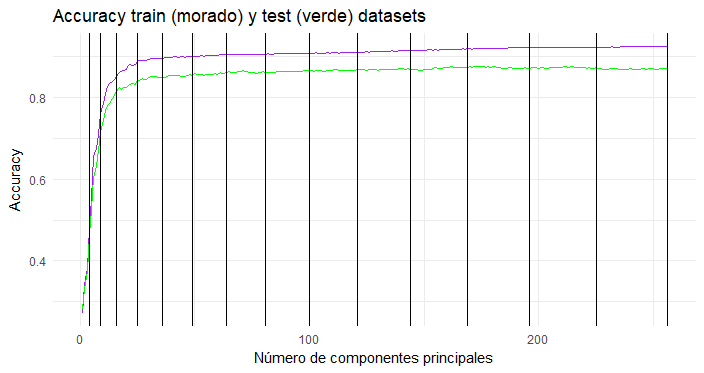
\includegraphics[scale=.7]{error.png}
    \caption{error de clasificación en función del número de componentes utilizadas}
    \label{fig:errroes_PCR}
  \end{center}
\end{figure}

Realizando un zoom en la parte inicial de la figura anterior se nota que un valor de 50 componentes principales parece correcto para predecir, desde el 25 se ve bien pero aun 50 componentes es una gran ganancia sobre las 256 variables originales.

\begin{lstlisting}[style=customc,basicstyle=\scriptsize]
ggplot(resumen2, aes(x = p, y =Accuracy.train, color= p )) +geom_line(aes(colour=I('Purple') )) +
  geom_line(aes(x = p, y =Accuracy.test, colour =I('green'))) +
  theme_minimal() + ggtitle('Accuracy train (morado) y test (verde) datasets')+
  ylab('Accuracy') + xlab('Numero de componentes principales')+ xlim(c(5,100)) +
  geom_vline(xintercept=2**2) + 
  geom_vline(xintercept=3**2) +
  geom_vline(xintercept=4**2) +
  geom_vline(xintercept=5**2) +
  geom_vline(xintercept=6**2) +
  geom_vline(xintercept=7**2) +
  geom_vline(xintercept=8**2) +
  geom_vline(xintercept=9**2)
\end{lstlisting} 

\FloatBarrier
\begin{figure}[H]
  \begin{center}
    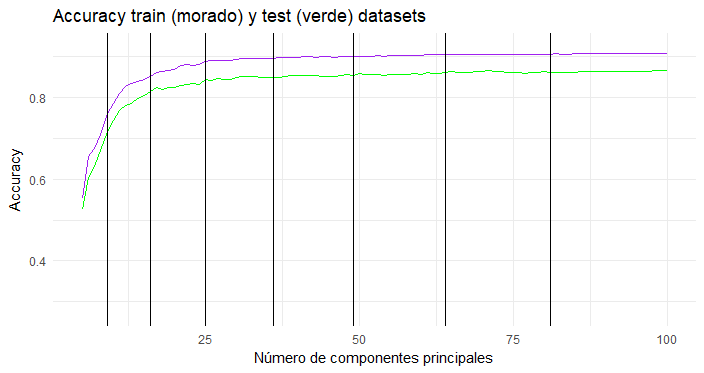
\includegraphics[scale=.7]{errores_zoom.png}
    \caption{error de clasificación en función del número de componentes utilizadas en el rango de $p\in [5,100]$ }
    \label{fig:errroes_PCR_zoom}
  \end{center}
\end{figure}

Así que solo utilizó las primeras 50 componentes principales y las guarda junto con los coeficientes de la regresión para poder evaluar, en la aplicación de shiny.\footnote{Por el uso del package ‘pixels’ no pude montar la aplicación en el servicio gratuito de shiny \url{http://www.shinyapps.io/} }

\begin{lstlisting}[style=customc,basicstyle=\scriptsize]
p <- 50
y_train <- train[,1]
y_train <- factor(y_train)
Y_train <- model.matrix(~y_train-1)
train$V1 <- NULL
pca <- princomp(train) #como los datos ya estan escalados en [-1, 1] uso la matriz de varianzas y covarianzas
z <- pca$loadings[,1:p]
Z <- as.matrix(train) *z #multiplicacion de matrices pero el tex lo marca como error
b <- lm(Y_train ~ . -1, data=as.data.frame(Z))
B <- b$coefficients
entrada <- runif(256, -1, 1)
Y.test.hat <-  entrada*z*B #multiplicacion de matrices pero el tex lo marca como error
which.max(Y.test.hat)
saveRDS(z,'componentes.rds')
saveRDS(B,'coeficientes.rds')
\end{lstlisting} 

Lo siguiente es el código de la app en shiny, interfaz gráfica 

\begin{lstlisting}[style=customc,basicstyle=\scriptsize]

##################################################
## Ejemplo que captura un numero y lo proyecta en los primeros
## 2 componentes principales previamente calculados en un
## conjunto de datos de entrenamiento y guardados en pc.rds
##################################################
library(shiny) 
library(shinythemes)
library(shinydashboard)
library(knitr)
library(markdown)

shinyUI(fluidPage(
  theme = shinytheme("cerulean"),
  h1("Calsificacion usando PCA!"),
  
  mainPanel(
    tabsetPanel(
      id = 'Clasificador',
      tabPanel('Prediccion usando PCR',
               tabItem(tabName="main",hr(), 
                       fluidRow( column(5, h4("Pinta el numero"),
                                        shiny_pixels_output( outputId = "pixels"),
                                        actionButton("captureDigit", "Capturar")
                       ),
                       column(5,h3("Numero reconocido como:"),
                              verbatimTextOutput("matriz") )))),
                       
      tabPanel("PCA",
               withMathJax(includeMarkdown('clasificador_PCR.md')))
        ),
      tabPanel("Doc de la app",
             tabItem(tabName="foo2",
                     withMathJax(includeMarkdown("app.md"))
                     
             ) 
    
    )
   )      
  )
\end{lstlisting} 


Y la parte del server


\begin{lstlisting}[style=customc,basicstyle=\scriptsize]
################################################
## Ejemplo que captura un numero y lo proyecta en los primeros
## 50 componentes principales previamente calculados en un
## conjunto de datos de entrenamiento y guardados en pc.rds
################################################
library(shiny) 
library(pixels)


shinyServer(function(input, output) 
{
  ## carga el objeto que contiene los PC calculados previamente
  z <- readRDS("C:/Users/fou-f/Desktop/MCE/Second/CienciaDeDatos/tarea1/ejercicio4/componentes.rds")
  ## coeficientes
  B <- readRDS('C:/Users/fou-f/Desktop/MCE/Second/CienciaDeDatos/tarea1/ejercicio4/coeficientes.rds')
  r.scale <- function(m)
  {
    #funcion para que la entrada de pixeles tenga la misma escala que los datos
    max <- max(m)
    min <- min(m)
    m <- ((m - min)/ (max - min)) # m \in [0,1]
    m*2-1     #asi m \in [-1, 1]
  }
  
  output$pixels <- shiny_render_pixels(
    show_pixels(grid=c(16,16), brush=matrix(c(1,1,1,1),2,2))) #obtencion de los pixeles
  
    output$prompt <- renderText("Dibuja un numero de una cifra")
    observeEvent(input$captureDigit, 
                 {
                   dig <<- (input$pixels)
                   data.digit <- matrix(dig,nrow=16,ncol=16,byrow=T)        
                   output$pixels <- shiny_render_pixels(
                            show_pixels(grid=c(16,16),
                          brush=matrix(c(.5,1,.5,1,1,1,.5,1,.5),3,3))
                            )
    output$matriz <- renderPrint({
      entrada <- r.scale(dig)
      proj <-entrada*z #multiplicacion de matrices pero el tex maraca error
      Y.hat.probs <- proj *B#multiplicacion de matrices pero el tex maraca error
      Y.hat <- which.max(Y.hat.probs)
      Y.hat <- Y.hat - 1 
      Y.hat
    })
    
    }) 
})
\end{lstlisting} 

\end{enumerate}
$$$$






\end{document}